\documentclass[10pt]{article}

\usepackage[version=3]{mhchem} % Package for chemical equation typesetting
\usepackage{siunitx,enumitem} % Provides the \SI{}{} and \si{} command for typesetting SI units
\usepackage{graphicx} % Required for the inclusion of images
\usepackage{natbib} % Required to change bibliography style to APA
\usepackage{nth}
\usepackage{amsmath} % Required for some math elements
\usepackage{tabulary} % table package
\usepackage{graphicx}
\usepackage{floatrow} % change the placement of table caption heading
\usepackage{float} % controls the placement of figures

\usepackage{chemfig} % use Chemistry symbols
\usepackage[font={small}]{caption}
\usepackage[margin=1in]{geometry}
\setlength\parindent{0pt} % Removes all indentation from paragraphs

% \renewcommand{\labelenumi}{\alph{enumi}.} % Make numbering in the enumerate environment by letter rather than number (e.g. section 6)

%\usepackage{times} % Uncomment to use the Times New Roman font


\title{Water Pollution\\ CHEM 1211L} % Title

\author{Chris \textsc{West}} % Author name

\date{\today} % Date for the report

\begin{document}

\maketitle % Insert the title, author and date

\begin{center}
\begin{tabular}{l r}
Date Performed: & June 19, 2017 \& June 21, 2017 \\% Date the experiment was performed
Partner: & Chris Tillis \\ % Partner names
Instructor: & Dr. MacGowan % Instructor/supervisor
\end{tabular}
\end{center}
\floatsetup[table]{capposition=top}
%\ce{Cu^2+}
\begin{abstract}
The objective of the Water Pollution experiment was to determine what filtering medium (approx. $2.00 g$) would be the most effective way in removing ``unknown polluted \ce{Cu} solution" and to determine its concentration level. As a class, each group was assigned to create one of the 6 ppm standards (1,3,5,7,9, \& 12) that would be used to create ``Beer's Law Calibration Plot for \ce{Cu^2+}" using AA. From the plot we get our trend line as $y = 0.1032x + 0.0255$ and our $R^2 = 0.99646$. Then using the AA again we took our group solutions and tested them to get it's absorbance values. Used those absorbance values and plugged it into the y from the ``Beer's Plot" trend line and got the x-values. From this we realized the most efficient medium was acid and the second most efficient was charcoal.
\end{abstract}
%----------------------------------------------------------------------------------------
%	SECTION 1
%----------------------------------------------------------------------------------------

\section{Data and Results of Calculations}
\begin{table}[H]
\label{Table 1}
\caption{Preparation of Polluted Water Samples}
\resizebox{30em}{!}{
\begin{tabular}{|l|l|l|}
\hline
\multicolumn{1}{|c|}{{\ul{\textbf{Type(s) of filtering media}}}} &
\multicolumn{1}{c|}{{\ul{\textbf{Mass of filtering material(grams)}}}} &
\multicolumn{1}{c|}{{\ul{\textbf{Vol. of the unknown polluted water sample (mL)}}}} \\ \hline
	Acid Exchange & 2.02 & 100.0 \\ \hline
	Carbon & 2.03 & 100.0 \\ \hline
	\end{tabular}
	}
	\centering
\end{table}

\begin{table}[H]
\label{Table 2}
\caption{Experimental parameters for analysis of polluted water samples by atomic spectroscopy}
\resizebox{50em}{!}{
\begin{tabular}{|l|l|l|l|l|}
\hline
\multicolumn{1}{|c|}{{\ul{\textbf{Wavelength (nm)}}}} &
\multicolumn{1}{c|}{{\ul{\textbf{Linear range (ppm)}}}} &
\multicolumn{1}{c|}{{\ul{\textbf{Flame typed used}}}} &
\multicolumn{1}{c|}{{\ul{\textbf{Blank used}}}} &
\multicolumn{1}{c|}{{\ul{\textbf{Copper stock solution concentration (ppm) used to prepare standards}}}} \\ \hline
	k \hline
	\end{tabular}
	}
	\centering
\end{table}

\begin{table}[H]
\label{Table 3}
\caption{Copper(II) ion Standards absorbance values and their corresponding concentration (ppm) at 324.7 wavelength}
\resizebox{20em}{!}{
\begin{tabular}{|l|l|}
\hline
\multicolumn{1}{|c|}{{\ul{\textbf{Concentration (ppm)}}}} &
\multicolumn{1}{c|}{{\ul{\textbf{Absorbance values}}}} \\ \hline
	1 & 0.115 \\ \hline
	3 & 0.318 \\ \hline
	5 & 0.553 \\ \hline
	7 & 0.786 \\ \hline
	9 & 0.964 \\ \hline
	12 & 1.234 \\ \hline
	\end{tabular}
	}
	\centering
\end{table}

\begin{table}[H]
\label{Table 4}
\caption{Absorbance values of polluted water sample and filtered polluted water samples}
\resizebox{10em}{!}{
\begin{tabular}{|l|l|}
\hline
\multicolumn{1}{|c|}{{\ul{\textbf{Name}}}} &
\multicolumn{1}{c|}{{\ul{\textbf{Absorbance}}}} \\ \hline
	Unknown (Straight up) & 1.873 \\ \hline
	1:10 Cu & 0.335 \\ \hline
	Charcoal (Straight up) & 0.665 \\ \hline
	Charcoal & 0.063 \\ \hline
	Acid (Straight up) & 0.367 \\ \hline
	\end{tabular}
	}
	\centering
\end{table}

\begin{table}[H]
\label{Table 5}
\caption{Experimental Results for the Remediation of Copper(II) ion from Polluted Water}
\resizebox{51em}{!}{
\begin{tabular}{|l|l|l|l|}
\hline
\multicolumn{1}{|c|}{{\ul{\textbf{Material}}}} &
\multicolumn{1}{c|}{{\ul{\textbf{Concentration (ppm) of \ce{Cu^2+} remaining}}}} &
\multicolumn{1}{c|}{{\ul{\textbf{Concentration (ppm) of \ce{Cu^2+} removed}}}} &
\multicolumn{1}{c|}{{\ul{\textbf{Efficiency for each filtering media (ppm/g)}}}} \\ \hline
    \ce{Cu} 1:10 & 29.99 &  & n/a \\ \hline
    Acid & 3.309 & 26.681 & 13.21 \\ \hline
    Charcoal & 6.197 & 23.793 & 11.72 \\ \hline

	\end{tabular}
	}
	\centering
\end{table}
%----------------------------------------------------------------------------------------
%	SECTION 2
%----------------------------------------------------------------------------------------
\section{Calculations \& Graph}
\begin{figure}[H]
\hfill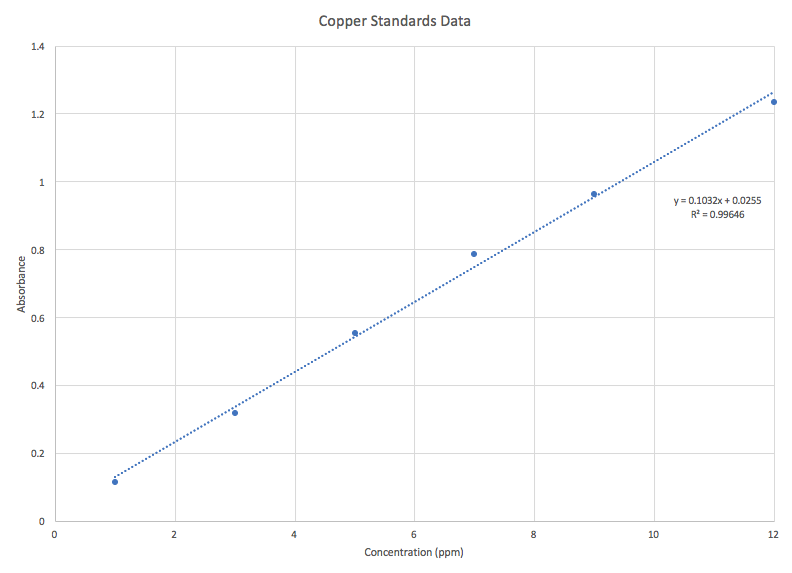
\includegraphics[width=5in]{fig1}\hspace*{\fill}
\caption[Beer's Law Calibration Plot for Copper(II) ions (ppm) by Atomic Absorption (324.7 nm)]{Beer's Law Calibration Plot for Copper(II) ions (ppm) by Atomic Absorption (324.7 nm)}
\end{figure}
Sample Calculation:

\begin{enumerate}[noitemsep]
    \item Preparation of a \ce{Cu^2+} standard from the stock solution
    \begin{itemize}
        \item Pipet 5.00 mL of 100ppm \ce{Cu^2+} into 100 mL volumetric flask.
        \item Dilute with 95 mL of water
        \item 5.00 mL $\times$ 100 ppm =$ C_2$ $\times$ 100 mL
        \item 5.00 mL $\times$ = $\frac{500 ppm*mL}{100.0 mL}$ = 5 ppm
    \end{itemize}
    \item Determination of \ce{Cu^2+} ppm for each filtrate
    \begin{itemize}
        \item Acid
        \begin{enumerate}
            \item y = 0.1032x + 0.0255
            \item y = Acid Absorbance = 0.367
            \item 0.367 = 0.1032x + 0.0255
            \item x = $\frac{0.367 - 0.0255}{0.1032}$ = 3.309 ppm
        \end{enumerate}
        \item Charcoal
        \begin{enumerate}
            \item y = 0.1032x + 0.0255
            \item y = Charcoal Absorbance = 0.665
            \item 0.665 = 0.1032x + 0.0255
            \item x = $\frac{0.665 - 0.0255}{0.1032}$ = 6.197 ppm
        \end{enumerate}
    \end{itemize}
    \item Determination of \ce{Cu^2+} in the unfiltered polluted water sample
    \begin{enumerate}
        \item y = 0.1032x + 0.0255
        \item y = \ce{Cu^2+} 1:10 = 0.335
        \item 0.335 = 0.1032x + 0.0255
        \item x = $\frac{0.335 - 0.0255}{0.1032}$ = 2.999 ppm
        \item 2.999 $\times$ 10 ( because of 1:10) = 29.99 ppm of unfiltered \ce{Cu^2+}
    \end{enumerate}
    \item Determination of the amount of \ce{Cu^2+} removed for each filtered medium
    \begin{itemize}
        \item Acid
        \begin{enumerate}
            \item 29.99 ppm - 3.309 ppm = 26.681 ppm
        \end{enumerate}
        \item Base
        \begin{enumerate}
            \item 29.99 ppm - 6.197 ppm = 23.793 ppm
        \end{enumerate}
    \end{itemize}
    \item Calculation of the efficiency
    \begin{itemize}
        \item Acid
        \begin{enumerate}
            \item $\frac{26.681 ppm}{2.02 g}$ = 13.21 ppm/g
        \end{enumerate}
        \item Charcoal
        \begin{enumerate}
            \item $\frac{23.793 ppm}{2.03 g}$ = 11.72 ppm/g
        \end{enumerate}
    \end{itemize}
\end{enumerate}
%----------------------------------------------------------------------------------------
%	SECTION 3
%----------------------------------------------------------------------------------------
\section{Questions}
In this experiment, we used a blank which was distilled water and dissolved \ce{Cu^2+} into it and it's purpose was to make sure our readings are correct. We simply chose it because we understood water's makeup. Using only the standards to create the Beer's Law plot we get a more accurate graph. If we were to use both the standards and filtrates we wouldn't have gotten an accurate graph. The reason we measure at $\lambda$ max for absorbance is this is where the most light is absorbed in a wavelength. The linear range for \ce{Cu} is $.15-12 ppm$. The linear range was used for the 6 different standards we had. By using a set range we create precise data and anything outside of the range would not be precise. A sample would have to be diluted if the absorbance was $>= 1$. The acid was most efficient filtering material with $13.21 ppm/g$. Using the previous module to solve this experiment is possible because both look for the absorbance values but the only difference would be how accurate one is to the other.
%----------------------------------------------------------------------------------------
%	SECTION 4
%----------------------------------------------------------------------------------------
\bibliographystyle{IEEEtran}
\begin{thebibliography}{1}
\bibitem{Chem}
Department of Chemistry and Physics (2015). \textit{Water Pollution and Remediation}. Armstrong State University, Savannah.
\end{thebibliography}
\end{document}
